\section{Evaluation}
\label{sec:evaluation}

In this section, we compare the performance of our EDP and CEDP algorithms
with that of the baseline placement policy defined in
Section~\ref{sec:motivate}.  Our evaluation consists of two parts: simulations
and testbed experiments, both of which are driven by real-world workloads. 

%The evaluation is composed of two parts, the simulation-based evaluation and
%the testbed-based one.  In the simulation part, we use two public datasets to
%drive the simulations, and the focuses of the simulations include analysis of
%the read imbalance problem and trade-offs in the design of EDP algorithm
%compared to the baseline algorithm.  We also compare the performances of
%baseline, EDP and CEDP in simulated hetegeneous setting.

%As for the testbed experiments, we mainly focus on the effects of various
%distribution algorithms on read latencies of files in a storage cluster with
%real-world configurations.  We use the Linux dataset only in the testbed
%experiments.  

%We observe that EDP and CEDP can outperform the baseline
%distribution method in storage clusters with homogeneous and heterogeneous
%network by 37.41\% and 52.12\%, respectively. {\bf PC: nowhere ???}

\subsection{Datasets}

%\begin{enumerate}
%\item FSLHOME 2013: 9 users, upto 90 backup versions, hash file only, variable chunking, detailed information on each file in the snapshot
%\item LINUX: Linux kernel developement repository backups uniformly sampled from 2.6.35 to current stable version. 
%\item SYNTHETIC: Not proper for this project because each backup is a single disk image of the backuped VM. The size of each backup is very large, and, under average 4KB chunking, the number of chunks of each backup is so large that the imbalance caused by deduplication can be mitigated.
%\end{enumerate}

We drive our evaluation using three public datasets:
\begin{itemize}
\item
{\em FSLHOME:} It is published by the File system and Storage Lab (FSL) at
Stony Brook University \cite{tarasov12}.  It contains daily snapshots of the
home directories of nine students on a shared network file system.  Each
snapshot comprises chunk fingerprints of multiple files obtained by
variable-size chunking.  Due to the large dataset size, we sample a subset of
snapshots in year 2013.  Our final FSLHOME dataset consists of a total of 104
snapshots, whose fingerprints are derived from the average chunk size of 4KB
using variable-size chunking. Each snapshot has 197K to 210K files.
%In the year 2013, the snapshots cover nearly daily backups of 9 active users
%from January 22 to June 17, and, for each user, we start from the first
%snapshot, and select the next snapshot if the gap of dates is larger than or
%equal to 7, i.e. one week.  Thus, the total number of snapshots of FSLHOME
%that we use in the evaluations is 104.  We pick the snapshots using
%variable-size chunking with 4KB average size in our evaluations.
\item
{\em LINUX:}  It contains 15 versions of {\em unpacked} Linux kernel source
code \cite{linux}, sampled from versions~2.6.35 to 3.16.3.  Each version has
size 393.77MB to 551.91MB of data with 30K to 50K files.  
\item
{\em LINUXTAR:}  It packs each version of the Linux kernel source code
\cite{linux} into a single tarball file.  It consists of 321 versions
of uncompressed tarballs.  Each tarball has size 4.93MB to 553.54MB of data.  
\end{itemize}

Our evaluation studies the backup scenario. In each backup operation, we store
a snapshot (for FSLHOME) or a version (for LINUX and LINUXTAR) and aim to
achieve read balance for the files within each backup based on
Problem~\ref{problem:gap}.  Note that the datasets are composed of different
file size distributions: both FSLHOME and LINUX comprise many small
files in each backup, while LINUXTAR contains one large tarball
file in each backup.  Thus, our evaluation addresses the impact of file size
distributions on read balance. 

%We sample every one out of 40 versions (one
%version is treated as one snapshot) from its master branch, starting from

%We use 4KB fixed-size chunking on LINUX and LINUXTAR to obtain chunk
%fingerprints in simulations and both fixed-size and variable-size chunking
%with 4KB average size in testbed experiments. 

For both FSLHOME and LINUX, we filter small files of size less than
16KB, so that we can distinguish more clearly the read balance gaps of
the data placement schemes based on the large files with enough numbers of
chunks.  These small files only account for 2.53\% and 5.84\% of total sizes
of FSLHOME and LINUX, respectively.  Note that there is no small
file in LINUXTAR.

%, and we can handle them separately by packing them into a single file.  
%After filtering the small files, 
The total logical sizes of FSLHOME, LINUX, and LINUXTAR are 6.46TB, 7.81GB,
and 101GB, respectively (after we filter the small files of FSLHOME and
LINUX).  The physical storage sizes of FSLHOME, LINUX, and LINUXTAR after
deduplication with 4KB variable-size chunking reduce to 0.34TB, 1.89GB, and
38.8GB, or equivalently, save 94.74\%, 75.8\%, and 61.50\% of disk space,
respectively.  If we use deduplication with 4KB fixed-size chunking for LINUX
and LINUXTAR, the savings are 70.04\% and 53.01\% disk space for LINUX and
LINUXTAR, respectively.
%(87.13\% for variable-size chunking).
%two reasons.  First, there are small performance differences on these files
%among different data placement policies.  Including the small files may 
%and EDP algorithm on these files while the large number of these files,
%around 89.30\% and 65.77\% of the total number of files in FSLHOME and
%LINUX, can
%ii) the total size of these files are small in each dataset, around 2.53\% of FSLHOME and 4.33\% of LINUX, and can be handled separately by packing them into a single file in upload/download.

%\subsection{Methodology}

%In both simulations and testbed experiments, we mainly compare performance of three types of distribution methods: i) baseline; ii) EDP and iii) CEDP.
%The major difference among the three methods lies in the way that they distribute the unique chunks of each file after deduplication.
%For each $k$ unique chunks, the baseline method randomly picks $n$ out of $N$ storage nodes and distributes the $n$ encoded chunks to the $n$ nodes in the round-robin fashion.
%The EDP method accumulates unique chunks of $t$ files in a buffer, solves the Problem~\ref{eq:normal_problem} using the Algorihtm~\ref{alg:edp} and distributes the unique chunks to the $N$ storage nodes following the output of the algorithm.
%The CEDP method is similar to the EDP method, but takes the heterogeneous download cost of each storage node into considerations in both the problem and the algorithm.
%
%In simulations, we mainly compare the write balance, read balance and degraded read balance in terms of number of chunks for baseline and EDP distribution methods.
%Even though the FSLHOME dataset is variable-size chunked, as there are large number of chunks in each snapshot and the average chunking size is fixed, we consider the number of chunks on each node as an approximation to the amount of data on each node.
%As for the LINUX dataset, as it is fixed-size chunked, the number of chunks is equivalent to the data size.
%In the testbed experiments, we mainly compare the read latency of each file for each distribution method.
%In both simulation-based and testbed-based evaluations, the results are averaged over 5 runs.

\subsection{Simulations}

\begin{figure}[H]
\centering 
\subfigure[FSLHOME]{
\includegraphics[width=4in]{trace_study/fsl_cdf.eps}
\label{fig:fsl_analysis}
}
\\
\subfigure[LINUX ]{
\hspace{0.1in}
\includegraphics[width=4in]{trace_study/linux_cdf.eps}
\label{fig:linux}
}
\\
\subfigure[LINUXTAR ]{
\hspace{0.1in}
\includegraphics[width=4in]{trace_study/linuxtar_cdf.eps}
\label{fig:linuxtar}
}
\vspace{-6pt}
\caption{Cumulative distributions of files versus performance gaps for the
baseline and EDP algorithms.}
\label{fig:trace_gap}
%\vspace{-6pt}
\end{figure}

%\begin{figure*}[!t]
%\centering 
%\subfigure[FSLHOME]{
%\includegraphics[width=2.2in]{trace_study/fsl_1_120_cdf.eps}
%\label{fig:fsl_analysis_hete}
%}
%\subfigure[LINUX ]{
%\hspace{-0.2in}
%\includegraphics[width=2.2in]{trace_study/linux_1_120_cdf.eps}
%\label{fig:linux_hete}
%}
%\subfigure[LINUXTAR ]{
%\hspace{-0.2in}
%\includegraphics[width=2.2in]{trace_study/linuxtar_1_120_cdf.eps}
%\label{fig:linuxtar_hete}
%}
%\vspace{-5pt}
%\caption{Cumulative distributions of files versus performance gaps for the
%baseline, EDP and CEDP in heterogeneous environment with link bandwidth 
%randomly distributed between [1,120]Mbps.}
%\vspace{-6pt}
%\end{figure*}

By default, our simulations consider a storage system with $N=16$ nodes, and
deploy $(n,k)=(14,10)$ erasure coding as in \cite{Sathiamoorthy13}.  We also
set $C = {16 \choose 14} \times 14\times 10 / 16 = 1,050$ (see
Section~\ref{sec:impl}) to balance the parity load.  For the chunking scheme,
we use 4KB variable-size chunking for FSLHOME, and 4KB fixed-size chunking for
LINUX and LINUXTAR.

\textbf{Effectiveness of EDP:} We analyze the read balance problem and answer
the following questions: (i) how severe read imbalance is in the baseline data
placement policy; and (ii) how well the EDP/CEDP algorithm tackles the
problem.  We start with the homogeneous setting.  We determine the chunk 
placements of the baseline and EDP algorithms based on chunk fingerprints 
and file metadata, and record the chunk distribution of each file.  We then 
calculate the read balance gap of each file using Equation~(\ref{eq:gap}).  

Figure~\ref{fig:trace_gap} plots the cumulative distributions of files versus
their gaps for FSLHOME, LINUX, and LINUXTAR.  For FSLHOME, the baseline only
keeps 22.59\% of files evenly distributed; and around 75\% of files have gaps
between 10\% and 50\%.  For LINUX, the baseline causes 42.95\% of files to
have gaps between 20\% and 80\%.  For LINUXTAR, the baseline causes 13.3\% of
files to have non-zero gaps.  On the other hand, EDP increases the percentage
of evenly distributed files in FSLHOME, LINUX, LINUXTAR to 90\%, 100\%, and
100\%, respectively. 

%{\color{red}Figures~\ref{fig:fsl_analysis_hete},~\ref{fig:linux_hete} and~ \ref{fig:linuxtar_hete} show the results in heterogeneous scenario. For all the three datasets, EDP and baseline has comparable performance as neither of them is aware of the heterogeneity in networks. For FSLHOME and LINUX, CEDP reduces the average gaps to 61.17\% and 58.90\%. For LINUXTAR, CEDP reduces gaps of 29.91\% of files to less than 50\%, and CEDP performs similarly to baseline on 70.09\% of files because these files have numbers of chunks larger than a distribution batch size and EDP enforces equal number of chunks to each storage node in a batch.}

%In FSLHOME dataset, we observe that not all files are evenly distributed by EDP algorithm, and this is because that EDP aims at minimizing the total gaps of distributions of chunks of files in a batch and may sacrifice the read balance of some files for the benefits of all the files in the batch.

%We summarize the results of this study as follows: i) In real-world storage
%clusters with deduplication, baseline distribution method causes distribution
%of chunks of large proportion of files unbalanced, and the imbalance ratio
%can be quite large; ii) EDP algorithm can balance the distribution of chunks
%for most of the backup files.  

%The distribution buffer size in our system for a real-world cluster with 16 storage nodes using (14,10) coding scheme is 16800, and, with the average number chunks of a file being around 8 in both FSLHOME and LINUX datasets, the average number of files in a distribution buffer is around 2000.


\begin{figure}[H]
\centering
\subfigure[ Read balance (FSLHOME) ]{
\includegraphics[width=4in]{balance/fsl_read_balance.eps}
\label{fig:fsl_readb}
}
%\subfigure[ Write balance (FSLHOME) ]{
%\includegraphics[width=2.2in]{balance/fsl_write_balance.eps}
%\label{fig:fsl_writeb}
%}
\\
\subfigure[ Degraded read balance (FSLHOME) ]{
\includegraphics[width=4in]{balance/fsl_degraded_balance.eps}
\label{fig:fsl_degradedb}
}
%\\
%\subfigure[ Read balance (LINUX) ]{
%\includegraphics[width=2.2in]{balance/read_balance.eps}
%\label{fig:readb}
%}
%\subfigure[ Write balance (LINUX) ]{
%\includegraphics[width=2.2in]{balance/write_balance.eps}
%\label{fig:writeb}
%}
%\subfigure[ Degraded read balance (LINUX) ]{
%\includegraphics[width=2.2in]{balance/degraded_balance.eps}
%\label{fig:degradedb}
%}
\vspace{-6pt}
\caption{Comparisons on read balance and degraded read balance between the
baseline and EDP algorithms. }
\label{fig:balance}
%\vspace{-6pt}
\end{figure}

\textbf{Impact of erasure coding:} We now study the read balance under
different values of the system size $N$ and erasure coding configurations
$(n,k)$.  We consider two read balance metrics: (i) read balance and (ii)
degraded read balance.  For degraded reads, we consider the single node
failure only (which is the common failure scenario
\cite{ford10,Sathiamoorthy13}), and simulate the failure by disabling the
first node.  We focus on the homogeneous setting, and compute both read
balance and degraded read balance metrics of the baseline and EDP algorithms
following Equation~(\ref{eq:gap}), in which we compute the gap as one minus
the ratio of the even number of read chunks of a file to the maximum number of
read chunks of the file over all nodes.  

%Note that we evaluate the read balance and degraded read balance metrics at the file level.   On the other hand, we compute the write balance gap at the snapshot level, in which it's defined as one minus the ratio of the even number of written chunks of a snapshot to the maximum number of written chunks of the snapshot over all nodes.  Each snapshot consists of multiple batches of chunks, in which the last batch may not be full. 

%We compare each type of balance of baseline and EDP algorithm as the scale of
%the simulated storage cluster increases.  For write balance, we upload each
%backup version of the dataset to the simulator, and calculate the imbalance
%ratio as the difference between the maximum and average number of number of
%chunks to distribute to a node over the average number of number of chunks to
%distribute to a node.  For normal read balance and degraded balance, we
%calculate the imbalance ratio using the number of chunks to download from
%each storage node.  For each system setting, we calculate the average
%imbalance ratio over all backup files.

%The degraded read balance indicates the balance level of distribution of the number of chunks to download from storage nodes in a degraded file read.
%The chunks in a degraded read include both the data chunks of the downloaded file and the code chunks in the same stripes as the unavailable data chunks.

%For write balance, we record the number of chunks that are distributed to each storage node in each backup, calculate the imbalance metric as 1-max/mean, and calculate the average imbalance metric for all backup versions.
%For normal read balance and degraded read balance, we record the number of chunks of a file to download from each storage node, using normal read and degraded read, respectively, and calculate the average imbalance metric of chunk numbers for all files.
%Note that, in the study of degraded read balance, we always set the first node as failed in the simulator before each file read.

We focus on FSLHOME, while the results for LINUX and LINUXTAR
are similar.  Figures~\ref{fig:balance} compares the read balance and
degraded read balance metrics for the baseline and EDP algorithms using
FSLHOME.  For read balance (see Figure~\ref{fig:fsl_readb}), the baseline
leads to high gaps that range between 20\% and 30\%, while EDP reduces the
gaps to 5\%.  EDP also keeps a smaller gap than the baseline in degraded read
balance (see Figures~\ref{fig:fsl_degradedb}). 


\begin{figure}[h]
\centering
\subfigure[ FSLHOME ]{
\includegraphics[width=4in]{hete/fsl_hete.eps}
\label{fig:fsl_hete}
}
\\
\subfigure[ LINUX ]{
\hspace{-0.1in}
\includegraphics[width=4in]{hete/hete.eps}
\label{fig:linux_hete}
}
\\
\subfigure[ LINUXTAR ]{
\hspace{-0.1in}
\includegraphics[width=4in]{hete/linuxtar_hete.eps}
\label{fig:linuxtar_hete}
}
\vspace{-6pt}
\caption{Read latency improvements of EDP and CEDP over baseline.}
\label{fig:sim_hete}
%\vspace{-15pt}
\end{figure}

\textbf{Impact of heterogeneity:} We simulate heterogeneous environments with
varying I/O bandwidths across nodes. We assume that the link bandwidths of
storage nodes follow a uniform distribution so as to simulate a distributed
storage environment \cite{li10}. 
Here,  we randomly assign the bandwidth to each node using four
uniform distributions: [1,120]Mbps, [10,120]Mbps, [30,120]Mbps, and
[60,120]Mbps.  We calculate the average improvement ratio of both EDP and CEDP
algorithms over the baseline for each file, in terms of the reduction of read
latency.  For CEDP, the weight $w_j~(1\le j \le 16)$ associated with each
storage node is set as the reciprocal of the I/O bandwidth of the node
(see Section~\ref{subsec:heterogeneity}).

%For each distribution range, we uniformly select a bandwidth value from the range, assign it to one of the 16 storage nodes, and run simulations on read performance using baseline, EDP and CEDP distribution algorithm on the simulated cluster.

%The x-axis indicates the 4 distribution ranges of link capacity, and the y-axis shows the average improvement ratio of file read latency of either EDP or CEDP algorithm over that of baseline distribution algorithm.
Figure~\ref{fig:sim_hete} shows the results.  When the I/O bandwidths are
highly varying, CEDP improves the baseline by 50.89\%, 48.90\%, and 42.55\% 
for FSLHOME, LINUX, and LINUXTAR, respectively, yet EDP shows very
small improvements.  For FSLHOME and LINUX, the improvements of EDP and CEDP 
become similar when the I/O bandwidths are less varying; for LINUXTAR, EDP is
almost identical to the baseline (which conforms to the results in
Figure~\ref{fig:linuxtar}), and CEDP improves the latency of both the baseline
and EDP.  Overall, CEDP remains robust in heterogeneous environments. 


%The trade-off is that EDP introduces a (slightly) higher gap in write balance
%(see Figure~\ref{fig:fsl_writeb}). The reason is that if a batch is not full 
%(e.g., the last batch of a snapshot), EDP may not write the same number of 
%chunks to each node.  Nevertheless, the gap is kept less than 5\% in all cases. 
%Thus, even though EDP requires to distribute equal number of chunks to storage nodes in a full batch write, it still trades off write balance for read balance when the batch cannot be fully filled.

% From this set of evaluations, we realize that EDP trades off write balance
% in each backup upload for better normal read balance of reading each
% uploaded file.  In addition, the degraded read balance of EDP is also
% improved compared to baseline.


%As the distribution range of link capacity decreases, the improvement ratio
%in read latency of CEDP over baseline decreases.  For EDP, when the
%transmission bandwidths are between 1Mbps and 120Mbps, read performance of
%EDP and baseline is the same.  As the distribution range decreases, the
%improvement ratio in read latency of EDP over baseline increases because the
%storage cluster is getting homogeneous.

%\item \emph{Analyze the imbalance problem}: Traces: FSL and Linux; Upload all backups of the trace to simulator, and then download all the files. For each file, calculate its maximum number of chunks to download from a storage node, and compare the numbers under baseline and EDP schemes to that in the theoretical even distribution to show that: i) baseline will suffer a lot from the imbalance problem; ii) EDP can achieve near-optimal distribution for read balance.

%\item \emph{EDP Algorithm Overhead}: Compare metadata processing time of baseline and EDP algorithm with two settings: i) upload single file, with the number of chunks of the file $\in \{1024,4096,16384,65540\}$; ii) upload multiple file of 64 chunks, with the number of files $\in \{16, 32, 64, 128, 256, 512, 1024\}$. As mentioned in the Section~\ref{sec:algorithm}, both number of chunks and number of files contribute to the complexity of the EDP algorithm, we want to evaluate the write performance of EDP for different types of workload. For this simulation, I plan to generate synthetic files using /dev/urandom with specific size and number.


%\item \emph{Write Balance}: Compare the number of data chunks (including parity chunks) that are distributed to each node by baseline and EDP algorithm. I plan to fix the stripe size as 8, parity number as 2, and set the number of storage nodes in the set \{10,12,14,16,18\}. I will compare the difference in write balance of baseline and EDP as the number of storage node varies. Trace: Linux

%\item \emph{Read Balance}: Similar to "analyze the imbalance problem", but here I plan to configure $n$ in the range \{9,10,11,12,13\} and $k$ in the range \{6,7,8,9,10\} while $m$ is fixed as 2. I will upload the trace to the simulator using either baseline or EDP scheme, and calculate the average performance difference in read balance, i.e. difference in maximum number of chunks to download from a node, of the two schemes under each configuration. I plan to show the result in two graphs, one with x-axis of $n$ ranging in the above range, and y-axis shows how the difference changes and the other one with x-axis of $k$ ranging in the above range, and y-axis shows how the difference changes. Target trace: Linux

%\item \emph{Heterogeneous Environement}: Comparison between EDP and CEDP for various uniform distributions of link capacities. \textit{Design:}  Link bandwidth of each node is uniformly distributed between [1,120], [3,120], [10,120], [30,120], [60,120] and [100,120]Mbps. Plot the average improvement ratio in file read of CEDP over EDP. \textit{Plot:} Type: barchart; x: range of link bandwidth distribution; y: improvement ratio( or average download time) Target trace: linux

%\item \emph{Degraded Reads}: Upload all the files of a trace to the simulator, kill the first slave node, and compare the read balance of baseline and EDP in degraded reads. Show the results similar to that in "Read Balance" part.


%\textbf{Benchmark} We first benchmark the download performance of our proto-type, and want to show that network transmission is the bottleneck in file read.
%To verify the bottleneck of network transmission, we configure the storage cluster with 1 master node and 8 slave nodes.
%One client uploads 1GB unique data to the storage cluster, and then downloads the 1GB file from the cluster.
%We measure the bottleneck download latency among the 8 storage nodes while the link capacities of all the storage nodes are configured as 10Mbps, 100Mbps and 1Gbps.
%The benchmark results are shown in Table~\ref{tab:bench_download}.
%The first row indicates the link capacity of each of the storage node, the second row shows the maximum transmission latency of the 8 storage nodes in a file read and the third row is the total file read latency, starting from initiation of download request to completion of reconstructing the downloaded file.
%Note that the transmission latency includes not only the data transmission latency, but also the request transmission latency and disk I/O latency at the slave side.
%First, we observe that the transmission latency dominates the total file read latency.
%In addtion, we realize that, as the per node link capacity increases from 10Mbps to 100Mbps and from 100Mbps to 1000Mbps, the transmission latency decreases.
%This implies that, in either case, network transmission is the bottleneck in file read, compared to disk I/O.
%Thus, in the testbed experiments, to accelerate the experiments rate and ensure network as the bottleneck, we configure each storage node with 100Mbps link capacity.
%\begin{table}[!t]
%\caption{Prototype Download Benchmark.}
%\centering
%\label{tab:bench_download}
%\begin{tabular}{|c||c|c|c|}
%\hline
% Link Capacity (Mbps)        &   $10$  &  $100$     &   $1000$  \\
%\hline
% Transmission Latency (sec) & $116.00$ & $12.17$ & $9.73$   \\
%\hline
% Read Latency (sec) & $116.26$ & $12.42$ & $9.98$   \\
%\hline
%\end{tabular}
%\end{table}

%\emph{To show:} \par
%1) The baseline upload is bottlenecked by chunking and network transmission;\par
%2) Overhead of EDP/CEDP upload compared to baseline;\par
%3) The baseline download is bottlenecked by the link bandwith at client side.

%\emph{Plan:} \par
%1) Upload 1GB unique data with single client to the system using baseline distribution. Evaluate the chunking time, metadata processing time, data transmission time; \par
%2) Upload 1GB unique data with single client to the system using EDP/CEDP distribution. Evaluate the chunking time, metadata processing time and data transmission time. Compare the metadata processing time with that of baseline; \par
%3) Download the 1GB unique data file using single client. Evaluate the download throughput.


%\emph{Design:} For each backup version, download all uploaded files by a single client. Calculate the average improvement ratio in download time of EDP over baseline. \textbf{Time estimation here: For linux trace, around 8 hours for one run, including EDP and baseline} \par
%\emph{Chart:} x: backup version; y: improvement ratio. \par
%\emph{Improvement Ratio:} For one file, the improvement ratio is (download latency of baseline-download latency of EDP)/(download latency of baseline). And the average improvement ratio is the average of the ratios for all downloaded files.

%\textbf{Heterogeneity}
%\emph{Design:} Totally 16 slave nodes, 5 with 1Gbps, 6 with 100Mbps and 5 with 10Mbps. Upload trace to the system using BASELINE, EDP and CEDP respectively. Download all the uploaded files for each backup version, and calculate the average improvement ratio in file read latency of CEDP over BASELINE and EDP over BASELINE. \par
%\emph{Plot:} Type: barchart; x: backup version; y: improvement ratio
\subsection{Testbed Experiments}
\label{subsec:testbed}

We evaluate via testbed experiments the read performance of various data
placement algorithms using our prototype in Section~\ref{sec:impl}.  Our
testbed consists of one client node, one metadata server node, and 16 storage
nodes.  We run each node on a multi-core machine, and interconnect all
machines via a Gigabit Ethernet switch.  The machines have varying CPU,
RAM, and harddisk configurations.  Here, we configure environments where the
network transmission is the bottleneck.   In a homogeneous setting, all nodes
are configured with 100Mbps link bandwidth; in a heterogeneous setting, we
configure five storage nodes with 10Mbps link bandwidth, six storage nodes
with 100Mbps link bandwidth, and the five remaining storage nodes with 1Gbps
link bandwidth.  The client node and master node are configured with 1Gbps
link bandwidth.  All nodes run Ubuntu 12.04.2 with Linux kernel 3.5. 

%The client node, master node and 11 of the slave nodes are with Intel
%Quad-Core 3.4GHz CPU, 8GB RAM and one ST1000DM003 7200RPM 1TB SATA disk while
%the rest 5 slave nodes are with Intel Dual-Core 2.13GHz CPU, 2GB RAM and one
%ST3160815AS 7200RPM 160GB SATA disk.  We have verified that the various CPU,
%RAM and disk configurations at slave side will not affect the
%bottlenecked network transmission, and, as long as the link capacity of
%each storage node is identical, we consider such cluster homogeneous.

We mainly focus on LINUX and LINUXTAR so as to evaluate both
fixed-size and variable-size chunking schemes.  Both chunking schemes choose
4KB as the chunk size.  The client writes each version, ordered by the version
number, to the prototype.   After that, the client reads all files of each
version and records the read latency.  We compute the normalized read latency
of each file using EDP or CEDP with respect to that of the same file using the
baseline.  We then compute the average normalized latencies of all files.  For
CEDP, we set the weight $w_j~(1\le j \le 16)$ associated with each storage
node as the reciprocal of the link bandwidth of the node.  The testbed results
are averaged over five runs.

\begin{figure}[H]
\centering
\subfigure[ Homogeneous, fixed-size chunking ]{
\includegraphics[width=4in]{testbed/testbed_linux.eps}
%\caption{Average download improvement of EDP over BASELINE for each backup version of Linux dataset.}
\label{fig:testbed_homo}
}
\\
\subfigure[ Homogeneous, variable-size chunking ]{
\includegraphics[width=4in]{review/testbed/testbed_linux.eps}
%\caption{Average download improvement of EDP over BASELINE for each backup version of Linux dataset.}
\label{fig:testbed_homo_var}
}
\\
\subfigure[ Heterogeneous, fixed-size chunking ]{
\includegraphics[width=4in]{hete/testbed_hete.eps}
%\caption{Average download improvement of CEDP over BASELINE and EDP over BASELINE for each backup version of Linux dataset in heterogeneous network.}
\label{fig:testbed_hete}
}
\\
\subfigure[ Heterogeneous, variable-size chunking ]{
\includegraphics[width=4in]{review/testbed/testbed_linux_hete.eps}
%\caption{Average download improvement of CEDP over BASELINE and EDP over BASELINE for each backup version of Linux dataset in heterogeneous network.}
\label{fig:testbed_hete_var}
}
\vspace{-6pt}
\caption{Average normalized read latency for files of LINUX.}
\end{figure}

\begin{figure}[H]
\centering
\subfigure[ Homogeneous, LINUX 3.16.3]{
\includegraphics[width=4in]{testbed/testbed_linux_latency.eps}
\label{fig:testbed_homo_latency}
}
\\
\subfigure[ Heterogeneous, LINUX 3.16.3]{
\hspace{20pt}
\includegraphics[width=4in]{testbed/testbed_linux_hete_latency.eps}
\label{fig:testbed_hete_latency}
}
\\
\subfigure[ Heterogeneous, LINUXTAR ]{
\hspace{8pt}
\includegraphics[width=4in]{review/testbed/linuxtar_hete_latency.eps}
%\caption{Average download improvement of EDP over BASELINE for each backup version of Linux dataset.}
\label{fig:tar_hete_latency}
}
\caption{Read latency distributions of Linux 3.16.3 and LINUXTAR (the files in
the x-axis are sorted by the order that they are written to the prototype).}
%\caption{Read latency of files in version 3.16.3.}
%\vspace{-15pt}
\label{fig:latency}
\end{figure}

%Here, the x-axis indicates the kernel version, and the y-axis is the average normalized read latency of files in a kernel version.
{\bf Impact of chunking schemes:}  We compare the read latency results for
both fixed-size and variable-size chunking schemes.  In the interest of space,
we only present the results of LINUX.
Figures~\ref{fig:testbed_homo} and \ref{fig:testbed_homo_var} show the results
in the homogeneous testbed for both chunking schemes.   On average, EDP
reduces the read latency of the baseline by 37.41\% and 21.38\% for fixed-size
and variable-size chunking schemes, respectively.  We see that the normalized
read latency of EDP is higher with variable-size chunking. The reason is that 
in variable-size chunking, the read latency may be determined by some chunks
that have size larger than the average chunk size.  This reduces the
performance gap between EDP and the baseline. 

%Note that EDP has higher read latency in the first Linux version 2.6.35,
%since the first version has a smaller deduplication saving and the impact
%of duplicate chunks on the read balance is smaller. 

Figures~\ref{fig:testbed_hete} and \ref{fig:testbed_hete_var} present the
results in the heterogeneous testbed.  EDP is agnostic about heterogeneity. 
Its read latency reduction over the baseline drops to 22.12\% for fixed-size
chunking; even worse, it increases the read latency of the baseline by 10.79\%
for variable-size chunking.  CEDP addresses the issue by taking into account
the heterogeneous bandwidths.  It reduces the averaged read latency over the
baseline by 52.11\% and 25.74\% for fixed-size and variable-size chunking
schemes, respectively. 

%Figures~\ref{fig:testbed_homo} and \ref{fig:testbed_hete} show the results of 
%{\color{red} LINUX using fixed-size chunking on} the homogeneous and
%heterogeneous testbeds, respectively.  We see that in the
%homogeneous testbed (see Figure~\ref{fig:testbed_homo}), EDP reduces the read
%latency by an average of 37.41\%.  Note that for the first Linux version
%2.6.35, the read latency of EDP is close to that of the baseline because the
%first snapshot has a low storage saving due to deduplication, so the impact of
%duplicate chunks on read balance is small.  In a heterogeneous testbed (see
%Figure~\ref{fig:testbed_hete}), the read latency of EDP is 77.88\% of that of
%the baseline.  With the heterogeneity awareness, CEDP places chunks
%proportionally to the link bandwidth of each storage node, and its average
%read latency reduces to around 47.89\% of that of the baseline (i.e., CEDP
%reduces the read latency of the baseline by 52.11\%). 

%{\color{red} We also evaluate the read performance using 4KB variable-size chunking 
%(see Figures~\ref{fig:testbed_homo_var} and~\ref{fig:testbed_hete_var}). EDP can 
%reduce average latency to 76.27\% of that of baseline in homogeneous testbed while 
%CEDP can save up to 30.78\% read latency of baseline in heterogeneous testbed. 
%One difference in result using variable-size chunking is that, in heterogeneous testbed, 
%EDP induces 10.68\% more average read latency than baseline,
%which implies its deficiency in handling distribution in heterogeneous clusters.}

{\bf Read latency distribution:} We further examine the actual read latency
distributions, as shown in Figure~\ref{fig:latency}.   
Figures~\ref{fig:testbed_homo_latency} and \ref{fig:testbed_hete_latency} show 
the read latency distributions for the files in the last Linux version 3.16.3
using fixed-size chunking in both homogeneous and heterogeneous testbeds,
respectively.  In general, EDP improves the read latency for most of the files
compared to the baseline in homogeneous prototype (see
Figure~\ref{fig:testbed_homo_latency}); in the heterogeneous prototype, CEDP
reduces the read latency compared to both the baseline and EDP for most files 
(see Figure~\ref{fig:testbed_hete_latency}). 
Figure~\ref{fig:tar_hete_latency} shows the read latency distributions for all
321 versions in LINUXTAR.  CEDP outperforms the baseline by
35.74\%, and can save up to 10 seconds for some backup versions. 

\subsection{Computational Overhead}
\label{subsec:overhead}

EDP improves file read performance at the cost of extra computational
overhead on the write path compared to the baseline.  We evaluate the
computational overhead of EDP by measuring the processing time of determining
the placement of unique chunks in a batch.  We conduct our evaluation on a
machine with an Intel CPU at speed 3.4GHz.  We evaluate processing 
time by generating unique chunks with {\tt /dev/urandom} and feeding a batch of 
unique chunks to the EDP algorithm for processing.  We vary the number 
of files inside the batch from $1$ to $2,400$.  We assume that each file is of
equal size. 

Figure~\ref{fig:file_num} shows the processing times of the baseline and EDP
algorithms with different numbers of files.  As the number of files increases,
the processing time of EDP increases at a rate faster than that of the
baseline, since its complexity is quadratic to the number of files (see
Section~\ref{subsubsec:complexity}).  Nevertheless, the processing time
remains small.  For example, with 960 files, the average processing time of
EDP is around 0.20s; if the chunk size is 4KB, the processing throughput is
around 328.13MB/s.  We can further increase the throughput, for example, by
parallelizing the EDP algorithm.
%{\color{red} Practically, EDP algorithm should not bottleneck the backup
%process as there are much less than $1,000$ files in batches of our
	%evaluations.  In addition, small files could be packed together
	%before backup to accelerate EDP processing.}
%The processing time increases to 3.72 seconds 
%when there are 5600 files in a batch. With 4KB average chunk size, the processing 
%throughput of 1200 files is around 300MB/s while that of $5,600$ files drops to 17.64
%MB/s. The average numbers of files of LINUX and FSLHOME in a distribution batch 
%consisting of $N*C = 1260*16 = 20160$ chunks are 211 and 1580, respectively. Therefore, 
%EDP algorithm should not be the bottleneck on the write path. To sustain the processing 
%time of EDP, one possible approach is to dynamically adjust the batch size so that the 
%number of files is less than $1,000$. In addition, the SWAP step of EDP can be skipped for 
%files small imbalance ratio. We consider these accelerations as future works.}

%\begin{table}[!t]
%\caption{Number of files in distribution batch}
%\vspace{5pt}
%\centering
%\label{tab:num_files}
%\begin{tabular}{ccc}
%\toprule
%& FSLHOME & LINUX \\\toprule
%MEAN & 211.373 & $1,580.15$\\\toprule
%95-th & 267 & $4,090$\\\bottomrule
%\end{tabular}
%\end{table}

\begin{figure}[H]
\centering
\hspace{20pt}
\includegraphics[width=4in]{overhead/file_num.eps}
\caption{Batch processing time of the baseline and EDP with various numbers of
files in a batch.}
\label{fig:file_num}
\end{figure}



%which is much faster than current I/O bandwidth.
%As mentioned in Section~\ref{sec:algorithm}, two factors affect the processing time of EDP the most: i) the total number of chunks in a batch; ii) the total number of files in a batch.
%We compare the processing time of EDP and baseline in two settings to study the effect of the two factors.
%In the first setting, we fix the number of files as 1 in a batch, and vary the number of unique chunks of the file from 2160 up to 54720.
%In the second setting, we fix the number of unique chunks in a batch as 20160, and vary the number of files in the batch from 1 up to 960.
%Each file in the batch has the same number of chunks.
%Note that, in this evaluation, each file is generated using /dev/urandom device to ensure that all the chunks are unique.

%And we observe that the processing time of EDP and baseline are the same, and they both increase as the number of chunks increases.
%We observe that the number of files has little effect on the processing time of baseline distribution algorithm, but, for EDP algorithm, the processing time increases as the number of files in a batch increases.
%The reason is that the \textsc{InterFileAdjustment} step in EDP algorithm introduces the quadratic factor in terms of the number of files into the complexity.
%Based on our evaluation, with 960 files in a batch, the average processing time of EDP is around 0.20 second, and, with 4KB chunking size, the processing throughput is around 400MB/s, which is much faster than current I/O capacity.
%In addition, the average numbers of chunks per file in the LINUX and FSLHOME dataset are around 40 and 145, respectively, and, therefore, the average number of files in a batch is smaller than 500, which can be processed fast enough by EDP.

